\section{Results}\label{sec:results}

\subsection{Weighted Goal Programming Solution}
The model selected Dams 18, 19, and 23 with a total cost of \$481.5M. Relative to the ten goals, the solution exceeds several targets (e.g., height, capacity) while minimizing the weighted penalty of deviations, resulting in a weighted deviation score of 14.93. We can observe from Figure \ref{fig:wgpDeviationsChart} that the farmland area criterion was the driving factor in the WGP solution, with dam height and rainfall also exerting a significant influence. These three criteria together shaped the final weighted deviation score of 14.93. Table \ref{tab:model_results} lists per-dam attributes; Table \ref{tab:wgpAcheivementVsTarget}    summarizes achieved values versus targets and the corresponding deviations. This indicates a balanced compromise solution under the specified weights and budget.

\begin{figure}[htbp]
\centering
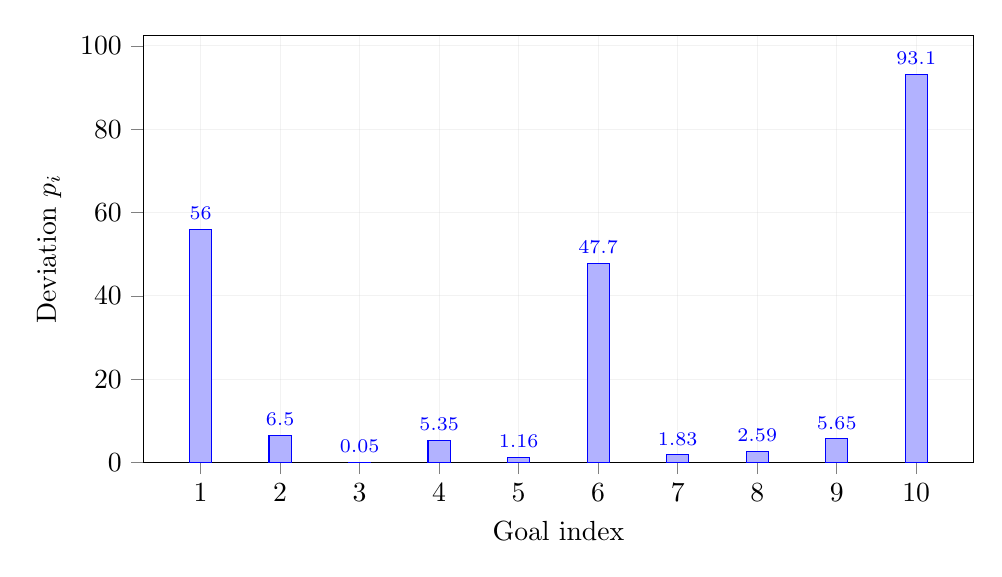
\begin{tikzpicture}
\begin{axis}[
    ybar,
    ymin=0,
    width=\textwidth,
    height=7cm,
    bar width=8pt,
    enlarge x limits=0.08,
    ylabel={Deviation $p_i$},
    xlabel={Goal index},
    xtick=data,
    xticklabel style={/pgf/number format/precision=0},
    nodes near coords,
    nodes near coords align={vertical},
    every node near coord/.append style={font=\scriptsize, /pgf/number format/fixed},
    tick align=outside,
    tick pos=left,
    grid=both,
    grid style={opacity=0.2},
]
\addplot coordinates
{ (1,56.00) (2,6.50) (3,0.05) (4,5.35) (5,1.16)
  (6,47.70) (7,1.83) (8,2.59) (9,5.65) (10,93.10) };
\end{axis}
\end{tikzpicture}
\caption{Weighted Goal Programming — deviations above targets ($p_i$) for each goal.}
\label{fig:wgpDeviationsChart}
\end{figure}

\begin{table}[htbp]
\centering
\caption{Goal achievement versus targets in the Weighted Goal Programming model}
\label{tab:wgpAcheivementVsTarget}
\begin{tabular}{clccc}
\hline
\textbf{\#} & \textbf{Criterion} & \textbf{Target} & \textbf{Achieved} & \textbf{Deviation} \\
\hline
1  & Dam height (m)        & 47.00   & 103.00   & $p_{1} = 56.00$ \\
2  & Capacity (Mm$^{3}$)   & 3.00    & 9.50     & $p_{2} = 6.50$  \\
3  & Reservoir area (km$^{2}$) & 0.04 & 0.09     & $p_{3} = 0.05$  \\
4  & Temperature ($^{\circ}$C) & 48.74 & 54.09   & $p_{4} = 5.35$  \\
5  & Population index      & 0.52    & 1.68     & $p_{5} = 1.16$  \\
6  & Rainfall              & 22.07   & 69.77    & $p_{6} = 47.70$ \\
7  & Residence             & 1.86    & 3.69     & $p_{7} = 1.83$  \\
8  & Farmland distance     & 0.32    & 2.91     & $p_{8} = 2.59$  \\
9  & Nearest road          & 0.23    & 5.88     & $p_{9} = 5.65$  \\
10 & Farmland area         & 0.68    & 93.78    & $p_{10} = 93.10$ \\
\hline
\end{tabular}
\end{table}


\subsection{Chebyshev Goal Programming Solution}
In the Chebyshev (min–max) goal programming run, we minimize the maximum normalized, weighted deviation across all ten goals, yielding an optimal scalar deviation of $ D^* = 25.2174$. Under the selection and budget constraints (exactly 3 dams, $\sum cost <= \$500$), the model selects dams 19, 20, and 28, with a total estimated cost of $\$158.7 + \$166.5 + \$172.1 = \$497.3$ million, thereby fully respecting the cap. Relative to the targets, this solution equalizes the worst-off goal (in the sense of the achievement scalarization), so no single criterion dominates the compromise. The binding deviations are those that attain $ D^*$ after normalization by their respective scaling factors, while the remaining goals exhibit strictly smaller normalized deviations. The binding criterion is Nearest road (Criterion 9) since it's weighted deviation $p_9/0.23 = 25.2174 = D^*$ (Table~\ref{tab:cgpWeightedDeviations}), all other deviations are strictly smaller. This indicates the worst normalized shortfall at the optimum occurs on the road-proximity goal, with all other goals at or within the Chebyshev bound. Detailed per-criterion achievements and deviations are reported in Table~\ref{tab:cgpAchievementVsTarget}, with the selected alternative attributes summarized in Table~\ref{tab:model_results}.

% =========================
% Table: cgpAchievementVsTarget
% =========================
\begin{table}[htbp]
\centering
\caption{CGP: goal achievement vs.\ targets and deviations (all $n_i=0$)}
\label{tab:cgpAchievementVsTarget}
\begin{tabular}{clcccc}
\hline
\textbf{\#} & \textbf{Criterion} & \textbf{Target} & \textbf{Achieved} & \textbf{Deviation type} & \textbf{Value} \\
\hline
1  & Dam height (m)              & 47.00   & 138.00  & $p_{1}$ & 91.00 \\
2  & Capacity (Mm$^{3}$)         & 3.00    & 71.50   & $p_{2}$ & 68.50 \\
3  & Reservoir area (km$^{2}$)   & 0.04    & 0.46    & $p_{3}$ & 0.42  \\
4  & Temperature ($^{\circ}$C)      & 48.74   & 48.74   & $p_{4}$ & 0.00  \\
5  & Population index            & 0.52    & 2.09    & $p_{5}$ & 1.57  \\
6  & Rainfall                    & 22.07   & 63.76   & $p_{6}$ & 41.69 \\
7  & Residence                   & 1.86    & 15.74   & $p_{7}$ & 13.88 \\
8  & Farmland distance           & 0.32    & 4.30    & $p_{8}$ & 3.98  \\
9  & Nearest road                & 0.23    & 6.03    & $p_{9}$ & 5.80  \\
10 & Farmland area               & 0.68    & 24.71   & $p_{10}$& 24.03 \\
\hline
\end{tabular}
\end{table}

\begin{table}[htbp]
\centering
\caption{Chebyshev GP: weighted deviations and the binding (max) constraint}
\label{tab:cgpWeightedDeviations}
\begin{tabular}{clccc}
\hline
\textbf{\#} & \textbf{Criterion} & \textbf{Deviation} & \textbf{Weight term in $D$} & \textbf{Weighted dev.} \\
\hline
3  & Reservoir area      & $p_3=0.4200$ & $\frac{1}{0.04}p_3$ & $10.5000$ \\
4  & Temperature         & $p_4=0$      & $\frac{1}{0.04}p_4$ & $0.0000$ \\
7  & Residence           & $p_7=13.8800$& $\frac{1}{22.07}p_7$& $0.6290$ \\
8  & Farmland distance   & $p_8=3.9800$ & $\frac{1}{0.32}p_8$ & $12.4375$ \\
9  & Nearest road        & $p_9=5.8000$ & $\frac{1}{0.23}p_9$ & \textbf{25.2174} \\
\hline
\multicolumn{4}{r}{\textbf{Max (i.e., $D^\star$)}} & \textbf{25.2174} \\
\hline
\end{tabular}
\end{table}


\subsection{Extended Goal Programming Solution}
% =========================
% EGP: one-paragraph summary (optional)
% =========================
In the Extended Goal Programming (EGP) run with $\alpha=0.8$, the model selects Dams $16$, $19$, and $28$ with a total estimated cost of $\$154.8+\$158.7+\$172.1=\$485.6$\,M (within the $\$500$\,M cap). The optimized bound on the Chebyshev-normalized terms is $D^\star=27.0$, while the composite objective value is $f^\star=\alpha D^\star + (1-\alpha)\!\left(\frac{p_3}{0.04}+\frac{p_4}{48.74}+\frac{p_7}{0.35}+\frac{p_8}{0.32}+\frac{p_9}{23}\right)=32.6816$. The $D$-binding criterion is \emph{Temperature} (criterion~4) because $\tfrac{p_4}{0.04}=27.0$ attains $D^\star$; the weighted-sum part is chiefly driven by \emph{Residence} via $\tfrac{p_7}{0.35}\approx 48.17$. Tables~\ref{tab:model_results} and \ref{tab:egpAchievementVsTarget} detail the selected alternatives and goal achievements; Fig.~\ref{fig:egpDeviations} visualizes both the $D$-normalized terms and the $(1-\alpha)$ weighted-sum terms for each criterion. 


% =========================
% Table: egpAchievementVsTarget
% =========================
\begin{table}[htbp]
\centering
\caption{EGP: goal achievement vs.\ targets and deviations (here, all $n_i=0$)}
\label{tab:egpAchievementVsTarget}
\begin{tabular}{clcccc}
\hline
\textbf{\#} & \textbf{Criterion} & \textbf{Target} & \textbf{Achieved} & \textbf{Deviation type} & \textbf{Value} \\
\hline
1  & Dam height (m)              & 47.00 & 98.00  & $p_{1}$  & 51.00  \\
2  & Capacity (Mm$^{3}$)         & 3.00  & 11.80  & $p_{2}$  & 8.80   \\
3  & Reservoir area (km$^{2}$)   & 0.04  & 0.10   & $p_{3}$  & 0.06   \\
4  & Temperature ($^{\circ}$C)    & 48.74 & 49.82  & $p_{4}$  & 1.08   \\
5  & Population index            & 0.52  & 50.82  & $p_{5}$  & 50.30  \\
6  & Rainfall                    & 22.07 & 50.10  & $p_{6}$  & 28.03  \\
7  & Residence                   & 1.86  & 18.72  & $p_{7}$  & 16.86  \\
8  & Farmland distance           & 0.32  & 2.09   & $p_{8}$  & 1.77   \\
9  & Nearest road                & 0.23  & 4.44   & $p_{9}$  & 4.21   \\
10 & Farmland area               & 0.68  & 45.24  & $p_{10}$ & 44.56  \\
\hline
\end{tabular}
\end{table}

% =========================
% Figure: egp_contribs
% Shows both D-normalized terms and (1-alpha) weighted-sum terms
% =========================
% Preamble needs:
% \usepackage{pgfplots}
% \pgfplotsset{compat=1.18}
\begin{figure}[htbp]
\centering
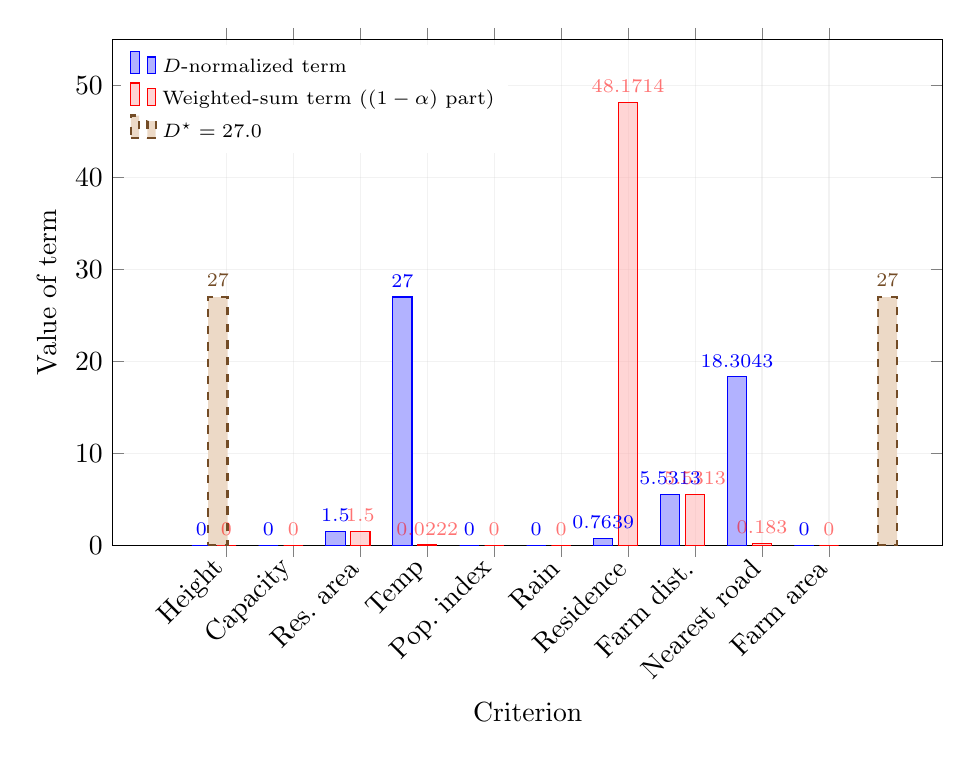
\begin{tikzpicture}
\begin{axis}[
    ybar,
    width=\textwidth,
    height=8cm,
    ymin=0,
    ymax=55, % accommodates the large p7/0.35 bar
    bar width=7pt,
    enlarge x limits=0.12,
    xlabel={Criterion},
    ylabel={Value of term},
    xtick=data,
    xticklabel style={rotate=45, anchor=east},
    xticklabels={
      Height,
      Capacity,
      Res.~area,
      Temp,
      Pop.~index,
      Rain,
      Residence,
      Farm~dist.,
      Nearest~road,
      Farm~area
    },
    legend style={draw=none, at={(0.01,0.99)}, anchor=north west, font=\scriptsize},
    legend cell align={left},
    nodes near coords,
    nodes near coords align={vertical},
    every node near coord/.append style={font=\scriptsize, /pgf/number format/fixed, /pgf/number format/precision=4},
    grid=both,
    grid style={opacity=0.2}
]
% --- Series 1: D-normalized terms (from the D-constraints) ---
% n1/47=0, n2/3=0, p3/0.04=1.5, p4/0.04=27.0, n5/48.74=0, n6/0.52=0,
% p7/22.07≈0.7639, p8/0.32=5.5313, p9/0.23≈18.3043, n10/0.68=0
\addplot+[fill] coordinates {
 (1,0.0000) (2,0.0000) (3,1.5000) (4,27.0000) (5,0.0000)
 (6,0.0000) (7,0.7639) (8,5.5313) (9,18.3043) (10,0.0000)
};
\addlegendentry{$D$-normalized term}

% --- Series 2: (1-$\alpha$) weighted-sum terms in the EGP objective ---
% Only present for p3, p4, p7, p8, p9 (others are zero here)
% p3/0.04=1.5, p4/48.74≈0.0222, p7/0.35≈48.1714, p8/0.32=5.5313, p9/23≈0.1830
\addplot+[fill, fill opacity=0.55] coordinates {
 (1,0.0000) (2,0.0000) (3,1.5000) (4,0.0222) (5,0.0000)
 (6,0.0000) (7,48.1714) (8,5.5313) (9,0.1830) (10,0.0000)
};
\addlegendentry{Weighted-sum term ($(1-\alpha)$ part)}

% Reference line at D*
\addplot+[domain=0.5:10.5, samples=2, thick, dashed] {27.0};
\addlegendentry{$D^{\star}=27.0$}
\end{axis}
\end{tikzpicture}
\caption{EGP contributions by criterion: comparison of the $D$-normalized terms (used in the minimax bound) versus the terms entering the $(1-\alpha)$ weighted-sum portion of the objective ($\alpha=0.8$). The $D$-binding criterion is \emph{Temperature}; the weighted-sum is dominated by \emph{Residence}.}
\label{fig:egpDeviations}
\end{figure}


\subsection{Lexicographic Goal Programming Solution}
In the Lexicographic Goal Programming (LGP) solution, we optimize three priority levels in sequence. \textbf{Priority~1} minimizes $(1/47)n_1+(1/3)n_2+(1/0.52)n_5+(1/0.68)n_{10}$ and attains $0$, implying no underachievement on height, capacity, population, or farmland area at the optimum. \textbf{Priority~2} then minimizes $(1/0.04)p_3+(1/48.74)p_4+(1/22.07)n_6$ subject to Priority~1’s optimum, yielding $0.0416$ (driven by temperature: $p_4/48.74\approx 0.0416$). \textbf{Priority~3} finally minimizes $(1/0.35)p_7+(1/0.32)p_8+(1/23)p_9$ under the earlier priorities, giving $83.4264$. The resulting portfolio selects Dams~\textbf{19, 21, 28} with total cost $\$158.7+\$164.3+\$172.1=\$495.1$\,M (within the \$500\,M cap). Table~\ref{tab:model_results} lists the attributes of the selected dams, and Table~\ref{tab:lgpAchievementVsTarget} reports achieved values versus targets and deviations; notably, temperature and the Priority~3 social–access criteria (residence, farmland distance, road proximity) drive the lexicographic refinement Figure \ref{fig:lgpPriorityThree}.

% =========================
% Table: lgpAchievementVsTarget
% =========================
\begin{table}[htbp]
\centering
\caption{LGP: goal achievement vs.\ targets and deviations (final portfolio; $n_i=0$)}
\label{tab:lgpAchievementVsTarget}
\begin{tabular}{clcccc}
\hline
\textbf{\#} & \textbf{Criterion} & \textbf{Target} & \textbf{Achieved} & \textbf{Deviation type} & \textbf{Value} \\
\hline
1  & Dam height (m)              & 47.00  & 123.00 & $p_{1}$  & 76.00 \\
2  & Capacity (Mm$^{3}$)         & 3.00   & 10.50  & $p_{2}$  & 7.50  \\
3  & Reservoir area (km$^{2}$)   & 0.04   & 0.04   & $p_{3}$  & 0.00  \\
4  & Temperature ($^{\circ}$C)    & 48.74  & 50.77  & $p_{4}$  & 2.03  \\
5  & Population index            & 0.52   & 1.13   & $p_{5}$  & 0.61  \\
6  & Rainfall                    & 22.07  & 55.60  & $p_{6}$  & 33.53 \\
7  & Residence                   & 1.86   & 26.02  & $p_{7}$  & 24.16 \\
8  & Farmland distance           & 0.32   & 4.80   & $p_{8}$  & 4.48  \\
9  & Nearest road                & 0.23   & 9.38   & $p_{9}$  & 9.15  \\
10 & Farmland area               & 0.68   & 36.41  & $p_{10}$ & 35.73 \\
\hline
\end{tabular}
\end{table}

% =========================
% Table: LGP priority objectives (tiny summary)
% =========================
\begin{table}[htbp]
\centering
\caption{Lexicographic GP: summary of priority objective values (final portfolio)}
\label{tab:lgpPriorityObjectives}
\begin{tabular}{clc}
\hline
\textbf{Priority} & \textbf{Objective minimized} & \textbf{Optimal value} \\
\hline
1 & $\frac{1}{47}n_1+\frac{1}{3}n_2+\frac{1}{0.52}n_5+\frac{1}{0.68}n_{10}$ & $0.0000$ \\
2 & $\frac{1}{0.04}p_3+\frac{1}{48.74}p_4+\frac{1}{22.07}n_6$               & $0.0416$ \\
3 & $\frac{1}{0.35}p_7+\frac{1}{0.32}p_8+\frac{1}{23}p_9$                    & $83.4264$ \\
\hline
\end{tabular}
\end{table}

% =========================
% Figure: Priority-3 terms bar chart
% =========================
% Preamble needs:
% \usepackage{pgfplots}
% \pgfplotsset{compat=1.18}
\begin{figure}[htbp]
\centering
\begin{tikzpicture}
\begin{axis}[
    ybar,
    width=\textwidth,
    height=7cm,
    ymin=0,
    ymax=75,
    bar width=12pt,
    enlarge x limits=0.2,
    xlabel={Priority 3 criteria},
    ylabel={Term value in objective},
    xtick=data,
    xticklabels={
      Residence $\big(\tfrac{1}{0.35}p_7\big)$,
      Farm dist. $\big(\tfrac{1}{0.32}p_8\big)$,
      Nearest road $\big(\tfrac{1}{23}p_9\big)$
    },
    nodes near coords,
    nodes near coords align={vertical},
    every node near coord/.append style={font=\scriptsize, /pgf/number format/fixed, /pgf/number format/precision=4},
    grid=both,
    grid style={opacity=0.2},
    legend style={draw=none, at={(0.02,0.98)}, anchor=north west, font=\scriptsize}
]
% Priority-3 weighted terms: p7/0.35, p8/0.32, p9/23
\addplot+[fill] coordinates {
 (1,69.0286) (2,14.0000) (3,0.3978)
};
\addlegendentry{Weighted term}

% (Optional) reference line at the total Priority-3 objective
\addplot+[domain=0.5:3.5, samples=2, thick, dashed] {83.4264};
\addlegendentry{Total $=83.4264$}

\end{axis}
\end{tikzpicture}
\caption{Lexicographic GP, Priority 3 objective components for the final portfolio: $\frac{1}{0.35}p_7=69.0286$, $\frac{1}{0.32}p_8=14.0000$, and $\frac{1}{23}p_9=0.3978$. Their sum equals the Priority 3 value $83.4264$.}
\label{fig:lgpPriorityThree}
\end{figure}


In Fig.~\ref{fig:lgpPriorityThree}, a clear pattern emerges. \textbf{Dam\~19} is selected by all four models, indicating a robust choice insensitive to the change from weighted-sum (WGP) to Chebyshev (CGP) to extended (EGP) and lexicographic (LGP) formulations. A near-core site, \textbf{Dam\~28}, appears in three models (CGP, EGP, LGP) but not WGP, suggesting that minimax and priority-based emphases favor it. The remaining slot is model-sensitive: WGP picks {18, 23}, CGP swaps in {20}, EGP prefers {16}, and LGP chooses {21}. Overall, moving from WGP to CGP/EGP/LGP consolidates consensus around {19, 28} while the third selection pivots according to each model’s treatment of deviations (weighted-sum vs.\ max-deviation vs.\ lexicographic priorities).

% Requires in preamble:
% \usepackage{pgfplots}
% \pgfplotsset{compat=1.18}

\begin{figure}[htbp]
\centering
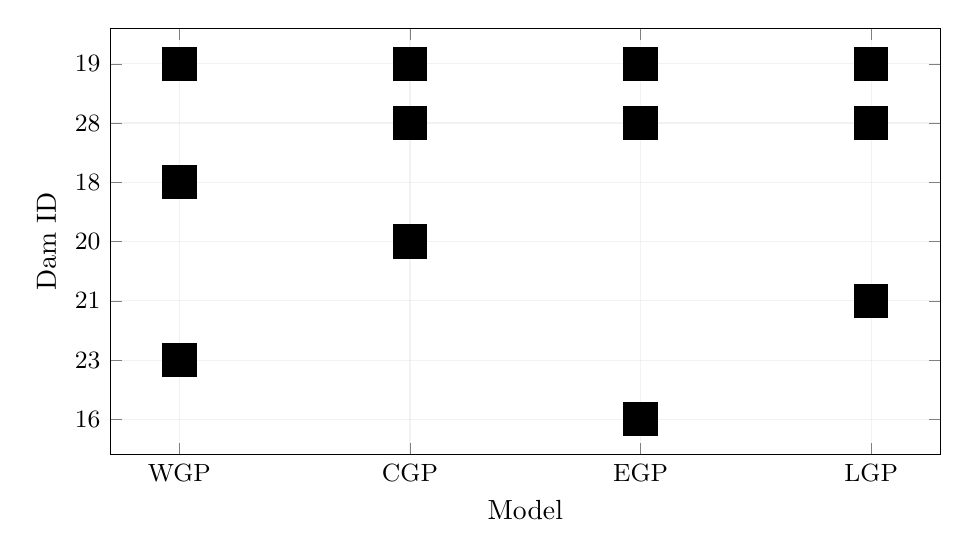
\begin{tikzpicture}
\begin{axis}[
  width=\textwidth,
  height=7cm,
  xlabel={Model},
  ylabel={Dam ID},
  xtick=data,
  ytick=data,
  symbolic x coords={WGP,CGP,EGP,LGP},
  symbolic y coords={19,28,18,20,21,23,16},
  y dir=reverse,
  grid=both,
  grid style={opacity=0.2},
  tick label style={font=\small},
]
\addplot[
  only marks,
  mark=square*,
  mark size=6pt
] coordinates {
  (WGP,19) (WGP,18) (WGP,23)
  (CGP,19) (CGP,20) (CGP,28)
  (EGP,19) (EGP,28) (EGP,16)
  (LGP,19) (LGP,28) (LGP,21)
};
\end{axis}
\end{tikzpicture}
\caption{Model–dam selection map for the four GP variants. Dam 19 is chosen by all four; Dam 28 by three (CGP, EGP, LGP); the others are singletons (WGP: 18, 23; CGP: 20; EGP: 16; LGP: 21).}
\label{fig:modelDamSelectionMap}
\end{figure}


\subsection{Multi-Choice GP Extension Solutions}
% In preamble:
% \usepackage{pgfplots}
% \pgfplotsset{compat=1.18}

\begin{figure}[htbp]
\centering
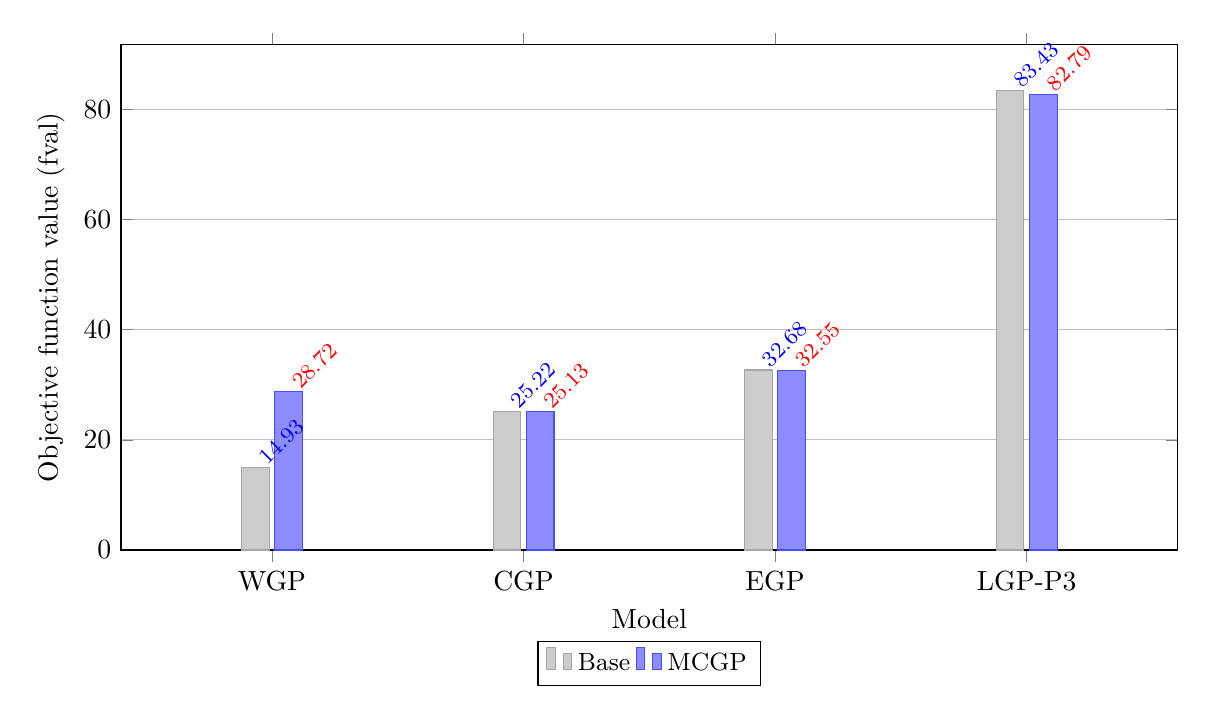
\begin{tikzpicture}
\begin{axis}[
  ybar,
  bar width=10pt,
  width=15cm,
  height=8cm,
  ymin=0,
  ylabel={Objective function value (fval)},
  xlabel={Model},
  symbolic x coords={WGP,CGP,EGP,LGP-P3},
  xtick=data,
  enlarge x limits=0.2,
  ymajorgrids,
  legend style={at={(0.5,-0.18)},anchor=north,legend columns=2,font=\small},
nodes near coords,
nodes near coords style={rotate=45, anchor=west, font=\footnotesize},
  every node near coord/.append style={font=\footnotesize}
]

% Base models
\addplot+[fill=gray!40, draw=gray!70]
  coordinates {(WGP,14.9277) (CGP,25.2174) (EGP,32.6816) (LGP-P3,83.4264)};
\addlegendentry{Base}

% MCGP
\addplot+[fill=blue!45, draw=blue!70]
  coordinates {(WGP,28.7245) (CGP,25.1304) (EGP,32.5462) (LGP-P3,82.7889)};
\addlegendentry{MCGP}

\end{axis}
\end{tikzpicture}
\caption{Comparison of \textit{fval} for Base vs.\ MCGP variants across models.}
\label{fig:fval_base_vs_mcgp}
\end{figure}

\begin{figure}[htbp]
\centering
\begin{tikzpicture}
\begin{axis}[
  title={Selected Dam Sites by Model: Base vs.\ MCGP},
  xlabel={Model / Variant},
  ylabel={Dam site ID},
  symbolic x coords={
    WGP--Base,WGP--MCGP,
    CGP--Base,CGP--MCGP,
    EGP--Base,EGP--MCGP,
    LGP-P3--Base,LGP-P3--MCGP
  },
  xtick=data,
  ymin=0, ymax=29,
  ytick={1,2,...,28},
  x tick label style={rotate=45,anchor=east,font=\small},
  width=16.5cm, height=9.5cm,
  grid=both, minor tick num=1
]

% All points same color (blue circles)
\addplot+[only marks, mark=*, mark options={fill=barfillbase, draw=barfillbase}, mark size=2.8pt]
  coordinates {
    % ---------- WGP ----------
    (WGP--Base,3) (WGP--Base,18) (WGP--Base,19)
    (WGP--MCGP,1) (WGP--MCGP,19) (WGP--MCGP,23)

    % ---------- CGP ----------
    (CGP--Base,19) (CGP--Base,20) (CGP--Base,28)
    (CGP--MCGP,19) (CGP--MCGP,20) (CGP--MCGP,28)

    % ---------- EGP ----------
    (EGP--Base,16) (EGP--Base,19) (EGP--Base,28)
    (EGP--MCGP,19) (EGP--MCGP,20) (EGP--MCGP,28)

    % ---------- LGP-P3 ----------
    (LGP-P3--Base,19) (LGP-P3--Base,21) (LGP-P3--Base,28)
    (LGP-P3--MCGP,19) (LGP-P3--MCGP,21) (LGP-P3--MCGP,28)
  };

\end{axis}
\end{tikzpicture}
\caption{Selected dam sites for each model under Base and MCGP formulations. All markers are blue circles; x-axis labels indicate the model variant.}
\label{fig:site_selection_base_vs_mcgp}
\end{figure}


\subsubsection{Weighted GP}
In the multi–choice extension of the weighted goal program (WGP–MCGP), five social/access criteria were allowed target flexibility. The model selected the lower bounds for \emph{Population} (0.52) and \emph{Farmland area} (0.68), while adopting the upper bounds for \emph{Nearest residence} (2.05), \emph{Farmland distance} (0.35), and \emph{Nearest road} (0.25), as shown in Table~\ref{tab:wgpMC_choices}. The resulting weighted deviation objective is $28.7245$, which is higher than the fixed–target WGP value ($14.9277$) by $+13.7968$ (Figure \ref{tab:wgpMCGPSummary}), reflecting the tighter upper–bound targets imposed on three criteria. Fig.~\ref{fig:wgpMC_intervals} visualizes the chosen target levels across the flexible goals and the model output is reported in \ref{tab:mcgpResult}.      

\begin{table}[htbp]
\centering
\caption{WGP–MCGP: flexible criteria, available targets, and chosen level (from $z$).}
\label{tab:wgpMC_choices}
\begin{tabular}{lccc}
\hline
\textbf{Criterion} & \textbf{Lower target (L)} & \textbf{Upper target (U)} & \textbf{Chosen} \\
\hline
Population index      & 0.52 & 0.57 & L (0.52) \\
Nearest residence     & 1.86 & 2.05 & U (2.05) \\
Farmland distance     & 0.32 & 0.35 & U (0.35) \\
Nearest road          & 0.23 & 0.25 & U (0.25) \\
Farmland area         & 0.68 & 0.75 & L (0.68) \\
\hline
\end{tabular}
\end{table}

% =========================
% Update to Table: WGP vs WGP–MCGP summary
% =========================
\begin{table}[htbp]
\centering
\caption{WGP vs.\ WGP–MCGP summary.}
\label{tab:wgpMCGPSummary}
\begin{tabular}{l l c c c}
\hline
\textbf{Model} & \textbf{Portfolio} & \textbf{Cost (M\$)} & \textbf{Objective} & \(\Delta\) vs.\ WGP \\
\hline
WGP (fixed targets)   & \{18,19,23\} & 481.5 & 14.9277 & -- \\
WGP–MCGP (flexible)   & \{1,19,23\}  & 487.4 & 28.7245 & +13.7968 \\
\hline
\end{tabular}
\end{table}

% Preamble: \usepackage{pgfplots} \pgfplotsset{compat=1.18}
\begin{figure}[htbp]
\centering
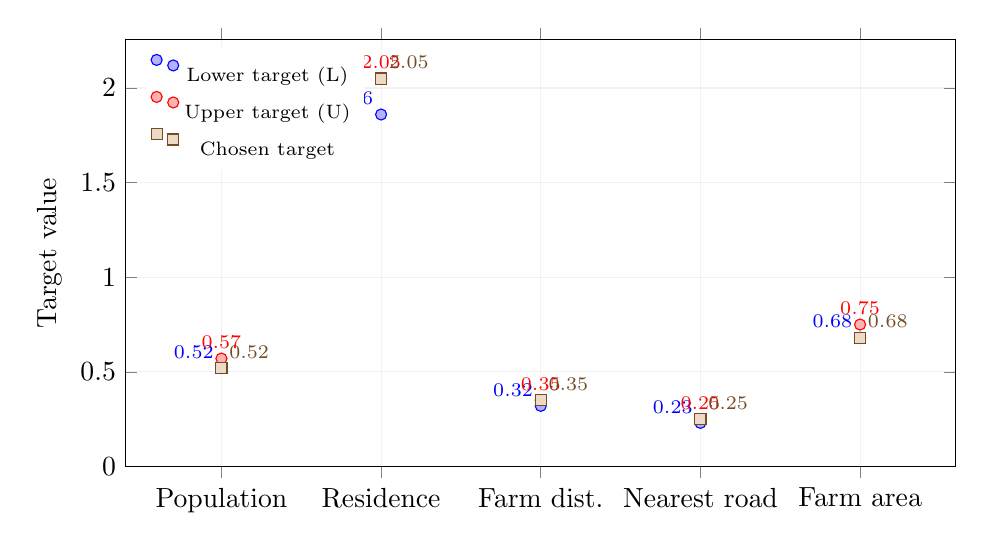
\begin{tikzpicture}
\begin{axis}[
  ybar=0pt,
  width=\textwidth, height=7cm,
  xtick=data,
  xticklabels={Population, Residence, Farm dist., Nearest road, Farm area},
  ylabel={Target value},
  ymin=0, enlarge x limits=0.15,
  grid=both, grid style={opacity=0.2},
  legend style={draw=none, at={(0.02,0.98)}, anchor=north west, font=\scriptsize},
  nodes near coords, nodes near coords align={vertical},
  every node near coord/.append style={font=\scriptsize}
]
% Lower targets (L)
\addplot+[mark=*, only marks] coordinates {(1,0.52) (2,1.86) (3,0.32) (4,0.23) (5,0.68)};
\addlegendentry{Lower target (L)}

% Upper targets (U)
\addplot+[mark=*, only marks] coordinates {(1,0.57) (2,2.05) (3,0.35) (4,0.25) (5,0.75)};
\addlegendentry{Upper target (U)}

% Chosen targets (from z) — plotted slightly above with square markers
\addplot+[mark=square*, only marks] coordinates {(1,0.52) (2,2.05) (3,0.35) (4,0.25) (5,0.68)};
\addlegendentry{Chosen target}
\end{axis}
\end{tikzpicture}
\caption{WGP–MCGP target flexibility across five criteria: chosen levels (squares) relative to the available lower/upper targets (dots).}
\label{fig:wgpMC_intervals}
\end{figure}


\subsubsection{Chebyshev GP}
Allowing target flexibility on five socio-environmental criteria retains the CGP portfolio $\{19,20,28\}$ while slightly improving the minimax objective from $D^{\star}\!=\!25.2174$ to $25.1304$ (Table~\ref{tab:cgpMCGPSummary}). The model chooses the lower targets for Population and Farmland area, and the upper targets for Nearest residence, Farmland distance, and Nearest road (Table~\ref{tab:cgpMCGPTargets}). With the selected dams, the worst normalized deviation is still \emph{Nearest road} ($p_9/0.23$), followed by Farmland distance and Reservoir area (Figure~\ref{fig:cgpMCGPDeviations}); all other normalized deviations are zero in the minimax sense. Achieved values relative to the chosen targets are detailed in Table~\ref{tab:cgpMCGPAchievementVsTarget} and the model output is reported in \ref{tab:mcgpResult}

% =========================
% CGP–MCGP: summary vs base CGP
% =========================
\begin{table}[htbp]
\centering
\caption{Chebyshev GP (CGP) vs. CGP–MCGP with target flexibility on five goals.}
\label{tab:cgpMCGPSummary}
\begin{tabular}{lcccc}
\toprule
Model & Selected dams & Total cost (M\$) & $D^\star$ & $\Delta D$ vs. CGP \\
\midrule
CGP (fixed targets)   & \{19, 20, 28\} & 497.3 & 25.2174 & -- \\
CGP--MCGP (flexible)  & \{19, 20, 28\} & 497.3 & 25.1304 & $-0.0870$ (–0.345\%) \\
\bottomrule
\end{tabular}
\end{table}
% =========================
% CGP–MCGP: chosen target levels (z)
% =========================
\begin{table}[htbp]
\centering
\caption{CGP--MCGP chosen targets for flexible goals (binary $z_k$: 1 = lower target, 0 = upper target).}
\label{tab:cgpMCGPTargets}
\begin{tabular}{llll}
\toprule
Criterion & Target options & Chosen ($z_k$) & Target used \\
\midrule
Population                 & $0.52$ (low) \;|\; $0.57$ (high) & $z_1=1$ & $0.52$ \\
Nearest residence          & $1.86$ (low) \;|\; $2.05$ (high) & $z_2=0$ & $2.05$ \\
Farmland distance          & $0.32$ (low) \;|\; $0.35$ (high) & $z_3=0$ & $0.35$ \\
Nearest road               & $0.23$ (low) \;|\; $0.25$ (high) & $z_4=0$ & $0.25$ \\
Farmland area              & $0.68$ (low) \;|\; $0.75$ (high) & $z_5=1$ & $0.68$ \\
\bottomrule
\end{tabular}
\end{table}
\input{charts/cgpMCGPDeviations.tex}
% =========================
% CGP–MCGP: goal achievement vs. chosen target
% =========================
\begin{table}[htbp]
\centering
\caption{CGP--MCGP achievements vs. (chosen) targets and deviations for the selected set $\{19,20,28\}$.}
\label{tab:cgpMCGPAchievementVsTarget}
\begin{tabular}{llrrl}
\toprule
\# & Criterion & Target & Achieved & Deviation \\
\midrule
1  & Height (m)                   & 47.00  & 138.00 & $p_1=91.00$ \\
2  & Capacity (Mm$^3$)            & 3.00   & 71.50  & $p_2=68.50$ \\
3  & Reservoir area (km$^2$)      & 0.04   & 0.46   & $p_3=0.42$ \\
4  & Temperature ($^{\circ}$C)    & 48.74  & 48.74  & $p_4=0.00$ \\
5  & Population (0--50, norm.)    & 0.52   & 2.09   & $p_5=1.57$ \\
6  & Rainfall (cm)                & 22.07  & 63.76  & $p_6=41.69$ \\
7  & Nearest residence (km)       & 2.05   & 15.74  & $p_7=13.69$ \\
8  & Farmland distance (km)       & 0.35   & 4.30   & $p_8=3.95$ \\
9  & Nearest road (km)            & 0.25   & 6.03   & $p_9=5.78$ \\
10 & Farmland area (km$^2$)       & 0.68   & 24.71  & $p_{10}=24.03$ \\
\bottomrule
\end{tabular}
\end{table} 

\subsubsection{Extended GP}
With $\alpha=0.8$, the extended goal program under multi-choice targets selects the same portfolio as the CGP--MCGP case, $\{19,20,28\}$, at a total cost of \$497.3\,M (Table~\ref{tab:egpMCGPSummary}). Target flexibility is exercised by choosing lower bounds for Population and Farmland area and upper bounds for Nearest residence, Farmland distance, and Nearest road (Table~\ref{tab:egpMCGPTargets}). The worst normalized deviation remains \emph{Nearest road} ($p_9/0.23=25.1304$), defining $D^{\star}$, followed by Farmland distance and Reservoir area (Figure~\ref{fig:egpMCGPDeviations}). The composite objective evaluates to $f=0.8\times 25.1304 + 0.2\times 62.2094 = 32.5462$, indicating that the portfolio balances a modest improvement in the minimax term with a larger weighted-sum contribution, consistent with the $\alpha$-weighted trade-off; per-criterion achievements and deviations are listed in Table~\ref{tab:egpMCGPAchievementVsTarget}.


% =========================
% EGP–MCGP: summary
% =========================
\begin{table}[htbp]
\centering
\caption{Extended Goal Programming with Multi-Choice targets (EGP--MCGP), $\alpha=0.8$.}
\label{tab:egpMCGPSummary}
\begin{tabular}{lccccc}
\toprule
Model & Selected dams & Total cost (M\$) & $D^{\star}$ & WGP term $S$ & Objective $f=\alpha D+(1-\alpha)S$\\
\midrule
EGP--MCGP & \{19, 20, 28\} & 497.3 & 25.1304 & 62.2094 & 32.5462 \\
\bottomrule
\end{tabular}
\end{table}


\input{tables/egpMCGPTargets.tex}
\input{tables/egpMCGPAchievementVsTarget.tex}
% =========================
% Figure: egpMC_deviations (normalized terms entering D)
% =========================
% Preamble needs:
% \usepackage{pgfplots}
% \pgfplotsset{compat=1.18}
\begin{figure}[htbp]
\centering
\begin{tikzpicture}
\begin{axis}[
    ybar,
    width=\textwidth,
    height=7cm,
    ymin=0,
    bar width=8pt,
    enlarge x limits=0.08,
    xlabel={Criterion (normalized term in $D$)},
    ylabel={Weighted deviation},
    xtick=data,
    xticklabel style={rotate=45, anchor=east},
    xticklabels={
      Height $(\tfrac{1}{47}n_1)$,
      Capacity $(\tfrac{1}{3}n_2)$,
      Res.~area $(\tfrac{1}{0.04}p_3)$,
      Temp $(\tfrac{1}{0.04}p_4)$,
      Pop. $(\tfrac{1}{48.74}n_5)$,
      Rain $(\tfrac{1}{0.52}n_6)$,
      Residence $(\tfrac{1}{22.07}p_7)$,
      Farm dist. $(\tfrac{1}{0.32}p_8)$,
      Nearest road $(\tfrac{1}{0.23}p_9)$,
      Farm area $(\tfrac{1}{0.68}n_{10})$
    },
    nodes near coords,
    nodes near coords align={vertical},
    every node near coord/.append style={font=\scriptsize, /pgf/number format/precision=4, /pgf/number format/fixed},
    grid=both,
    grid style={opacity=0.2},
    legend style={at={(0.02,0.98)},anchor=north west,draw=none,fill=none}
]
% Normalized deviations entering D:
% n1=0, n2=0, p3/0.04=10.5, p4/0.04=0, n5=0, n6=0, p7/22.07≈0.6203, p8/0.32=12.3438, p9/0.23=25.1304, n10=0
\addplot coordinates {
 (1,0.0000) (2,0.0000) (3,10.5000) (4,0.0000) (5,0.0000)
 (6,0.0000) (7,0.6203) (8,12.3438) (9,25.1304) (10,0.0000)
};
% Draw D* as a reference line
\addplot+[domain=0.5:10.5, samples=2] {25.1304};
\addlegendentry{$D^{\star}=25.1304$}
\end{axis}
\end{tikzpicture}
\caption{EGP--MCGP normalized deviations in the minimax term $D$. The binding criterion is \emph{Nearest road} with $p_9/0.23=D^{\star}$; next are Farmland distance and Reservoir area.}
\label{fig:egpMCGPDeviations}
\end{figure}

\subsubsection{Lexicographic GP}
Relative to the baseline LGP, introducing multi-choice targets leaves the Priority~1 and Priority~2 objectives unchanged while delivering a modest improvement at Priority~3 (from 83.4264 to 82.7889; Table~\ref{tab:LGPVsLGPMCObjectives}, Fig.~\ref{fig:LGPVsLGPMCObjectives}). The chosen target pattern is consistent across priorities—lower targets for Population and Farmland area, upper targets for Nearest residence, Farmland distance, and Nearest road (Table~\ref{tab:LPGMCGPTargets})—and the P1 portfolio is \{\LGPMCselPone\}, with the final P3 portfolio shown in Table~\ref{tab:LGP_LGPMC_selected_sets} and Fig. \ref{fig:lgpmc_selection_map}.


% =============================
% TABLE 1: Objectives by priority
% =============================
\begin{table}[htbp]
\centering
\caption{Lexicographic objectives by priority: baseline LGP vs LGP--MCGP.}
\label{tab:LGPVsLGPMCObjectives}
\begin{tabular}{lccc}
\toprule
{} & Priority 1 & Priority 2 & Priority 3 \\
\midrule
LGP (baseline)     & \LGPpOne  & \LGPpTwo  & \LGPpThree \\
LGP--MCGP (this work) & \LGPMCpOne & \LGPMCpTwo & \LGPMCpThree \\
\midrule
$\Delta$ (MCGP $-$ LGP) & 0.0000 & 0.0000 & -0.6375 \\
\bottomrule
\end{tabular}
\end{table}


% =============================
% TABLE 2: MCGP target choices (z) and used targets
% =============================
\begin{table}[htbp]
\centering
\caption{LGP--MCGP target flexibility (binary $z_k$: 1 = lower target, 0 = upper target).}
\label{tab:LPGMCGPTargets}
\begin{tabular}{llll}
\toprule
Criterion & Options & $z_k$ & Target used \\
\midrule
Population            & $0.52$ (low) \;|\; $0.57$ (high) & \zPop   & $0.52$ \\
Nearest residence (km)& $1.86$ (low) \;|\; $2.05$ (high) & \zRes   & $2.05$ \\
Farmland distance (km)& $0.32$ (low) \;|\; $0.35$ (high) & \zFarmD & $0.35$ \\
Nearest road (km)     & $0.23$ (low) \;|\; $0.25$ (high) & \zRoad  & $0.25$ \\
Farmland area (km$^2$)& $0.68$ (low) \;|\; $0.75$ (high) & \zFarmA & $0.68$ \\
\bottomrule
\end{tabular}
\end{table}
% =============================
% TABLE 3: Selected dam sets (IDs)
% =============================
\begin{table}[htbp]
\centering
\caption{Selected dam IDs across priorities.}
\label{tab:LGP_LGPMC_selected_sets}
\begin{tabular}{lll}
\toprule
Case & Priority & Selected dams (IDs) \\
\midrule
LGP (baseline)   & Final & \{\LGPbaseSel\} \\
LGP--MCGP        & P1    & \{\LGPMCselPone\} \\
LGP--MCGP        & P2    & \{\LGPMCselPtwo\} \\
LGP--MCGP        & P3    & \{\LGPMCselPthree\} \\
\bottomrule
\end{tabular}
\end{table}
% =============================
% TABLE 1: Objectives by priority
% =============================
\begin{table}[htbp]
\centering
\caption{Lexicographic objectives by priority: baseline LGP vs LGP--MCGP.}
\label{tab:LGPVsLGPMCObjectives}
\begin{tabular}{lccc}
\toprule
{} & Priority 1 & Priority 2 & Priority 3 \\
\midrule
LGP (baseline)     & \LGPpOne  & \LGPpTwo  & \LGPpThree \\
LGP--MCGP (this work) & \LGPMCpOne & \LGPMCpTwo & \LGPMCpThree \\
\midrule
$\Delta$ (MCGP $-$ LGP) & 0.0000 & 0.0000 & -0.6375 \\
\bottomrule
\end{tabular}
\end{table}


% =============================
% FIGURE: Selection map across priorities (no macros, fully explicit)
% Needs: \usepackage{pgfplots} \pgfplotsset{compat=1.18}
% =============================
\begin{figure}[htbp]
\centering
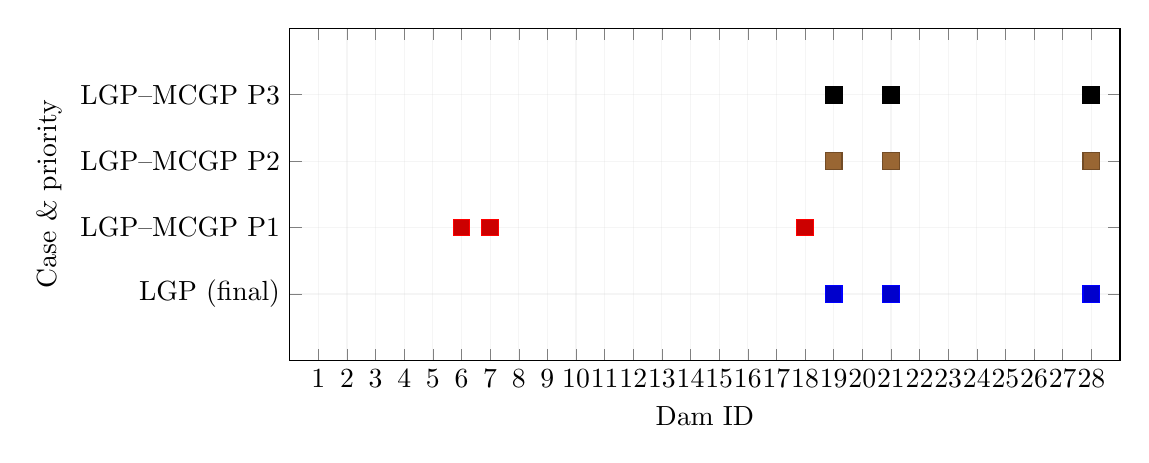
\begin{tikzpicture}
\begin{axis}[
  width=\textwidth, height=5.8cm,
  xmin=0, xmax=29, ymin=0, ymax=5, % integers -> robust parsing
  xlabel={Dam ID}, ylabel={Case \& priority},
  ytick={1,2,3,4},
  yticklabels={LGP (final), LGP--MCGP P1, LGP--MCGP P2, LGP--MCGP P3},
  xtick={1,2,...,28},
  grid=both, grid style={opacity=0.15},
  enlargelimits=false,
]

% Row 1: LGP (final) -> {19,21,28}
\addplot+[only marks,mark=square*,mark size=3pt]
  coordinates {(19,1) (21,1) (28,1)};

% Row 2: LGP–MCGP P1 -> {6,7,18}
\addplot+[only marks,mark=square*,mark size=3pt]
  coordinates {(6,2) (7,2) (18,2)};

% Row 3: LGP–MCGP P2 -> {19,21,28}
\addplot+[only marks,mark=square*,mark size=3pt]
  coordinates {(19,3) (21,3) (28,3)};

% Row 4: LGP–MCGP P3 -> {19,21,28}
\addplot+[only marks,mark=square*,mark size=3pt]
  coordinates {(19,4) (21,4) (28,4)};

\end{axis}
\end{tikzpicture}
\caption{Selected-dam map across LGP baseline and LGP–MCGP priorities. Filled squares mark dams included in each portfolio.}
\label{fig:lgpmc_selection_map}
\end{figure}



\subsection{Sensitivity Analysis}
Sensitivity analysis (SA) is a crucial step in multi-criteria decision-making (MCDM), as it evaluates the robustness of solutions when key model parameters are perturbed. In goal programming applications, where weights, targets, and other constraints guide the optimization, small changes can sometimes lead to disproportionately large shifts in the selected alternatives or in the overall objective performance. Testing models under these conditions therefore helps answer the central question: are the solutions stable enough to be trusted for real-world implementation, or do they fluctuate under modest changes in assumptions?

In this study, two types of sensitivity analysis were carried out to systematically investigate robustness across the four goal programming models considered—Weighted Goal Programming (WGP), Lexicographic Goal Programming (LGP), Chebyshev Goal Programming (CGP), and Extended Goal Programming (EGP).

We varied the distribution of weights across objectives using ten randomized test sets and compared the resulting solutions against the base model. The purpose was to determine whether changes in emphasis among objectives significantly alter the selection of dam sites or the associated objective function values. Key questions included: Which dam sites are consistently selected across different weight configurations? Which sites appear only under specific weight emphases? How variable are the objective values under weight perturbations?

Here, the emphasis shifted from weights to the target levels defined for each goal. Ten different target scenarios were generated and applied across all four models, with results compared against their respective base solutions. The objective was to assess: How sensitive is each model to adjustments in target values? Do some models show large swings in objective values while others remain stable? Which dam sites persistently appear across target variations, and which are target-sensitive?

Together, these analyses offer complementary insights. Weight SA reveals the impact of subjective trade-offs among competing objectives, while Target SA shows how solution stability depends on the feasibility and realism of the goals themselves. In the following sections, we first present the results of Weight SA, before moving on to Target SA.

\subsubsection{Weight Analysis}
The weight sensitivity analysis focused on how variations in the relative importance of objectives influenced the Weighted Goal Programming (WGP) and Lexicographic Goal Programming (LGP) models. Figure \ref{fig:weight_heatmap} maps dam-site selections across ten randomized weight sets compared with the base WGP solution. The heatmap shows that dams 18 and 19 were consistently chosen in nearly all scenarios, while other sites such as 12, 13, and 23 appeared only under specific weight allocations. This highlights the presence of a “core set” of robust sites that are insensitive to weight perturbations, alongside more marginal sites that enter solutions when emphasis shifts to particular objectives.

Objective function values also varied under weight perturbations. The lollipop plot in Figure \ref{fig:wgp_sa_lollipop_fval} compares the performance of each test set against the base WGP solution. While the base solution achieved an objective value of 14.93, the sensitivity runs produced substantially lower values ranging between 0.26 and 2.50. This suggests that, although the base configuration is balanced across objectives, certain weight allocations heavily prioritize specific goals at the expense of overall balance, yielding smaller numerical deviations. In other words, the weight distribution strongly shapes model efficiency, but the solutions remain internally consistent across scenarios.

A more direct measure of robustness is shown in the frequency analysis of dam selections (Figure \ref{fig:wgp_sa_frequency}). Dam 18 was selected in 70\% of runs, dam 19 in 80\%, and dam 23 in 60\%, while other sites appeared much less frequently. The overlay of the base solution confirms that the sites chosen there align with those most frequently selected under sensitivity runs, reinforcing the interpretation of robustness. Finally, the LGP model illustrates a different dynamic (Figure \ref{fig:lgp_fval_tradeoff}): while Priority 1 and Priority 2 objectives remain essentially stable across weight sets, Priority 3 shows wide variation, with objective values ranging from 2.5 to 13.1. This reflects the lexicographic structure—higher priorities dominate decision outcomes, leaving lower priorities sensitive to residual trade-offs. Together, these findings show that weight changes mainly affect the inclusion of marginal dam sites and the performance of lower-priority goals, while a stable subset of core sites persists across scenarios.

% Requires in preamble:
% \usepackage{pgfplots}
% \pgfplotsset{compat=1.18}

\begin{figure}[htbp]
\centering
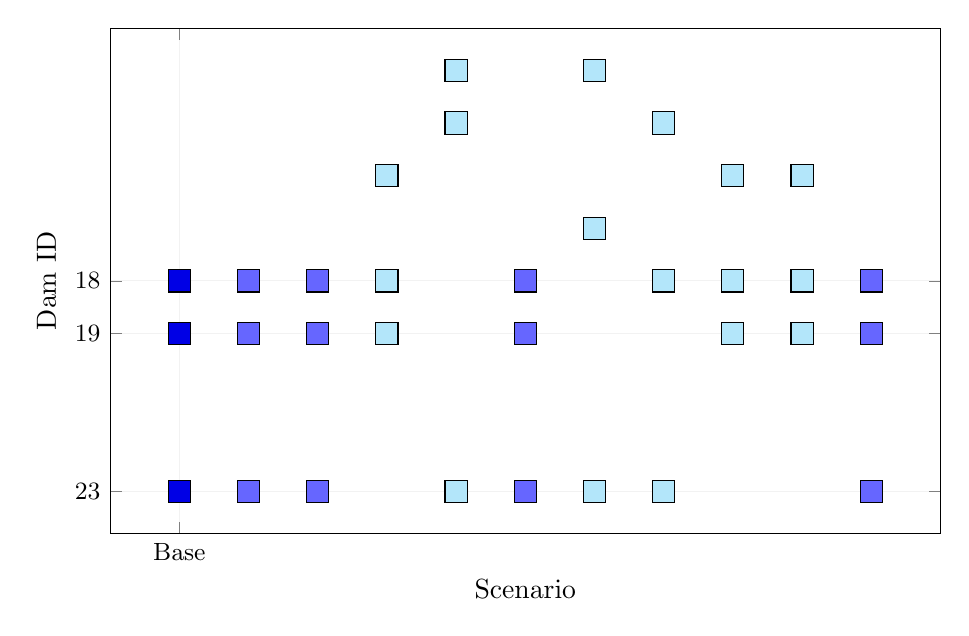
\begin{tikzpicture}
\begin{axis}[
  width=\textwidth,
  height=8cm,
  xlabel={Scenario},
  ylabel={Dam ID},
  xtick=data,
  ytick=data,
  symbolic x coords={Base,Test 1,Test 2,Test 3,Test 4,Test 5,Test 6,Test 7,Test 8,Test 9,Test 10},
  symbolic y coords={1,3,12,13,18,19,20,21,23},
  y dir=reverse,
  grid=both,
  grid style={opacity=0.2},
  tick label style={font=\small},
]
% Base (deep blue)
\addplot[
  only marks,
  mark=square*,
  mark size=4pt,
  draw=black,
  fill=blue!90!black
] coordinates {
  (Base,18) (Base,19) (Base,23)
};
% Matching Base selections in other scenarios (blue)
\addplot[
  only marks,
  mark=square*,
  mark size=4pt,
  draw=black,
  fill=blue!60
] coordinates {
  (Test 1,18) (Test 1,19) (Test 1,23)
  (Test 2,18) (Test 2,19) (Test 2,23)
  (Test 5,18) (Test 5,19) (Test 5,23)
  (Test 10,18) (Test 10,19) (Test 10,23)
};
% All other selections (light blue)
\addplot[
  only marks,
  mark=square*,
  mark size=4pt,
  draw=black,
  fill=cyan!30
] coordinates {
  (Test 3,12) (Test 3,18) (Test 3,19)
  (Test 4,1) (Test 4,3) (Test 4,23)
  (Test 6,1) (Test 6,13) (Test 6,23)
  (Test 7,3) (Test 7,18) (Test 7,23)
  (Test 8,12) (Test 8,18) (Test 8,19)
  (Test 9,12) (Test 9,18) (Test 9,19)
};
\end{axis}
\end{tikzpicture}
\caption{Scenario–dam selection map for the base WGP (first column) and ten test sets. Each filled square marks a selected dam site.}
\label{fig:weight_heatmap}
\end{figure}

\begin{figure}[htbp]
\centering
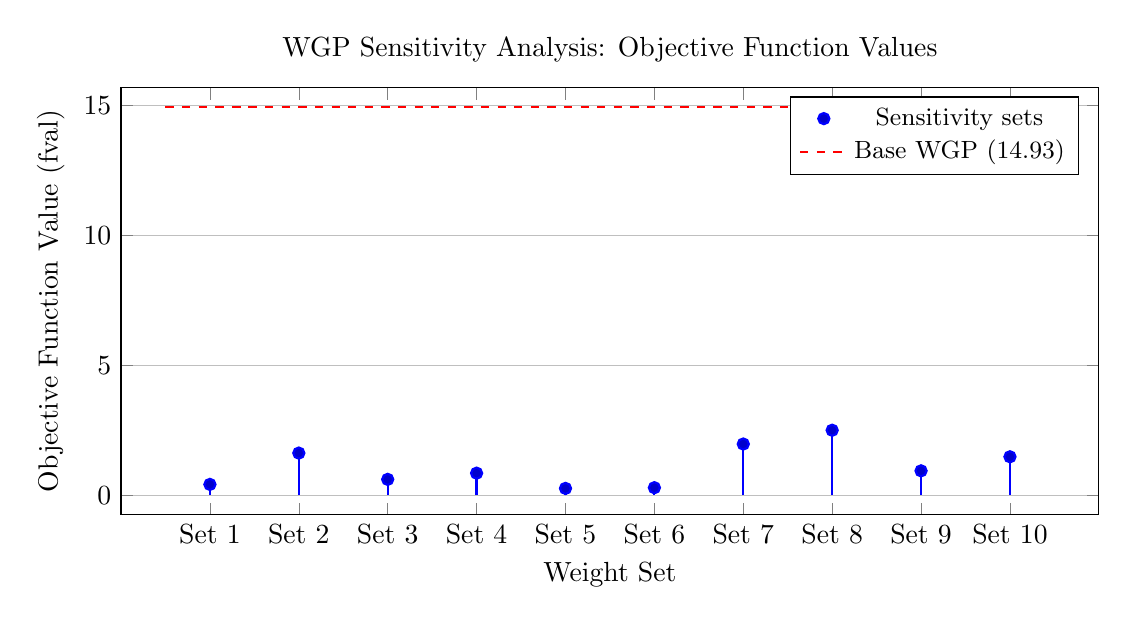
\begin{tikzpicture}
  \begin{axis}[
    title={WGP Sensitivity Analysis: Objective Function Values},
    xlabel={Weight Set},
    ylabel={Objective Function Value (fval)},
    xtick={1,2,3,4,5,6,7,8,9,10},
    xticklabels={Set 1, Set 2, Set 3, Set 4, Set 5, Set 6, Set 7, Set 8, Set 9, Set 10},
    width=14cm,
    height=7cm,
    ymajorgrids,
    ymin=0,
    enlargelimits=0.05,
    legend style={at={(0.98,0.98)},anchor=north east,font=\small},
  ]

  % Lollipop stems
  \addplot+[ycomb, mark=*, thick, blue] coordinates {
    (1,0.4128)
    (2,1.6183)
    (3,0.6062)
    (4,0.845)
    (5,0.2595)
    (6,0.286)
    (7,1.967)
    (8,2.4976)
    (9,0.935)
    (10,1.4761)
  };

  % Base WGP line
  \addplot[red, dashed, thick, domain=0.5:10.5] {14.9277};
  \addlegendentry{Sensitivity sets}
  
  \addlegendentry{Base WGP (14.93)}

  \end{axis}
\end{tikzpicture}
\caption{Lollipop plot of \textit{fval} across 10 weight sets (blue dots), compared with the base Weighted Goal Programming solution (red dashed line).}
\label{fig:wgp_sa_lollipop_fval}
\end{figure}

\begin{figure}[htbp]
\centering
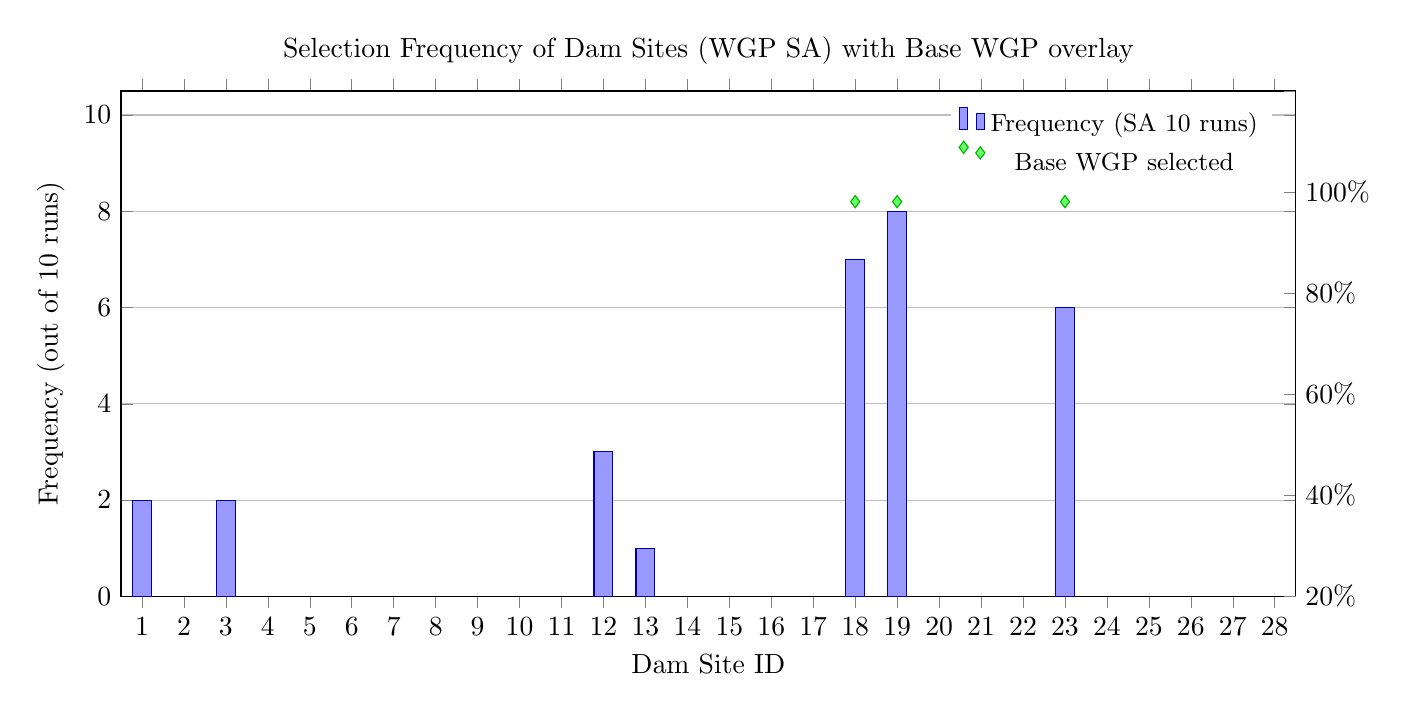
\begin{tikzpicture}

% =======================
% Left axis: Frequency bars (0..10)
% =======================
\begin{axis}[
  title={Selection Frequency of Dam Sites (WGP SA) with Base WGP overlay},
  xlabel={Dam Site ID},
  ylabel={Frequency (out of 10 runs)},
  ymin=0, ymax=10.5,
  xmin=0.5, xmax=28.5,
  xtick={1,2,...,28},
  width=16.5cm, height=8cm,
  ymajorgrids,
  bar width=0.45,
  ybar,
  legend style={font=\small, at={(0.98,0.98)}, anchor=north east, draw=none, fill=white},
]

% --- Frequency bars (hard-coded; 10 SA runs) ---
% Non-zero frequencies:
\addplot+[fill=blue!40!white, draw=blue!70!black] coordinates {
  (1,2) (3,2) (12,3) (13,1) (18,7) (19,8) (23,6)
};
\addlegendentry{Frequency (SA 10 runs)};

% --- Base WGP selections as red diamonds (placed slightly above max) ---
\addplot+[only marks, mark=diamond*, mark size=2.2pt, draw=green!70!black, fill=green!60] coordinates {
  (18,8.2) (19,8.2) (23,8.2)
};
\addlegendentry{Base WGP selected};

\end{axis}

% =======================
% Right axis: Percent labels (0..100%)
% =======================
\begin{axis}[
  hide x axis,
  axis y line*=right,
  ymin=0, ymax=10.5,
  ytick={0,2,4,6,8,10},
  yticklabels={0\%,20\%,40\%,60\%,80\%,100\%},
  width=16.5cm, height=8cm,
]
\end{axis}

\end{tikzpicture}
\caption{Summary of dam-site selection frequency across 10 WGP sensitivity runs; red diamonds mark sites selected by the Base WGP solution. Right axis shows percent of runs.}
\label{fig:wgp_sa_frequency}
\end{figure}
        
\begin{figure}[htbp]
\centering
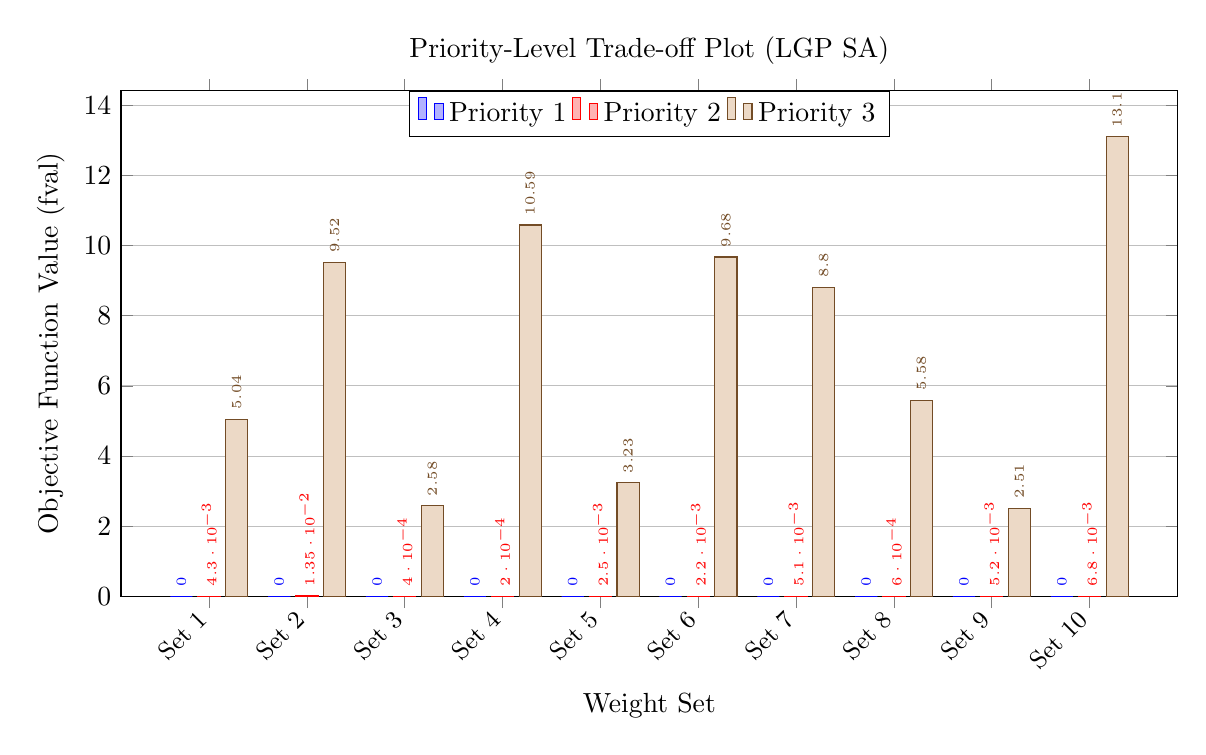
\begin{tikzpicture}
  \begin{axis}[
    ybar,
    bar width=8pt,
    title={Priority-Level Trade-off Plot (LGP SA)},
    xlabel={Weight Set},
    ylabel={Objective Function Value (fval)},
    symbolic x coords={Set 1,Set 2,Set 3,Set 4,Set 5,Set 6,Set 7,Set 8,Set 9,Set 10},
    xtick=data,
    xticklabel style={rotate=45,anchor=east,font=\small},
    width=15cm,
    height=8cm,
    ymin=0,
    enlarge x limits=0.1,
    legend style={at={(0.5,1)},anchor=north,legend columns=3},
    ymajorgrids,
    nodes near coords,
    nodes near coords align={vertical},
    every node near coord/.append style={font=\tiny, rotate=90, anchor=west}
  ]

  % Priority 1 (all zeros)
  \legend{Priority 1, Priority 2, Priority 3}
  \addplot coordinates {(Set 1,0) (Set 2,0) (Set 3,0) (Set 4,0) (Set 5,0) 
                        (Set 6,0) (Set 7,0) (Set 8,0) (Set 9,0) (Set 10,0)};
  % Priority 2
  \addplot coordinates {(Set 1,0.0043) (Set 2,0.0135) (Set 3,0.0004) (Set 4,0.0002) (Set 5,0.0025)
                        (Set 6,0.0022) (Set 7,0.0051) (Set 8,0.0006) (Set 9,0.0052) (Set 10,0.0068)};
  % Priority 3
  \addplot coordinates {(Set 1,5.0425) (Set 2,9.5191) (Set 3,2.5808) (Set 4,10.5879) (Set 5,3.2344)
                        (Set 6,9.6772) (Set 7,8.8018) (Set 8,5.5848) (Set 9,2.5091) (Set 10,13.1004)};

  \end{axis}
\end{tikzpicture}
\caption{Comparison of objective values (\textit{fval}) at Priority 1, 2, and 3 across weight sets for Lexicographic Goal Programming sensitivity analysis. Numbers above bars show exact values.}
\label{fig:lgp_fval_tradeoff}
\end{figure}



\subsubsection{Target Analysis}
The target sensitivity analysis investigated how variations in goal target levels affected model outcomes across the four formulations (WGP, CGP, EGP, and LGP). Figure \ref{fig:target_sa_linechart_with_base} shows the changes in objective values across ten target sets, compared with dashed lines representing the base models. WGP displayed remarkable stability, with values clustered tightly around its base of 14.93. LGP was also comparatively stable, with modest variation between 23 and 38. In contrast, CGP and EGP exhibited wide fluctuations: CGP ranged from 0.0 to 238.5, and EGP from 3.0 to 203.4. The logarithmic scale emphasizes these contrasts, highlighting that while WGP and LGP maintain consistent performance, CGP and EGP are highly sensitive to shifts in target definitions.

These variations are further reflected in dam-site selection patterns. Figure \ref{fig:dam_selection_targets_all_models} compares selected sites across models and target sets, with base solutions included for reference. WGP consistently selected the core set of dams 18, 19, and 20 across all scenarios, reflecting its stability under target perturbations. LGP displayed moderate variability, occasionally switching between site 19, 20, 21, and 28 depending on the target scenario. EGP and CGP were considerably more dynamic, with their selections shifting more frequently across sites such as 1, 16, 19, 20, and 28. This shows that while WGP and LGP preserve a degree of selection robustness, CGP and EGP yield more target-sensitive outcomes that may complicate interpretation and implementation.

Table \ref{tab:target_sa_stats} summarizes the descriptive statistics of objective values across the ten target scenarios for each model. WGP again emerges as the most stable (standard deviation = 0.63), followed by LGP (6.21), while CGP (87.44) and EGP (71.29) show very high variability. Finally, the grouped bar chart in Figure \ref{fig:target_sa_barplot_filtered} presents the frequency of site selection across target sets. The results reinforce the earlier patterns: dams 18–20 are robustly selected by WGP, dam 28 is highly persistent in LGP and partially in CGP/EGP, while sites such as 1, 15, 16, and 22 appear intermittently in the more sensitive models. Taken together, these findings demonstrate that target variation exerts strong influence on CGP and EGP, while WGP and LGP provide more stable recommendations and a clearer distinction between robust and target-sensitive dam sites.

\begin{figure}[htbp]
\centering
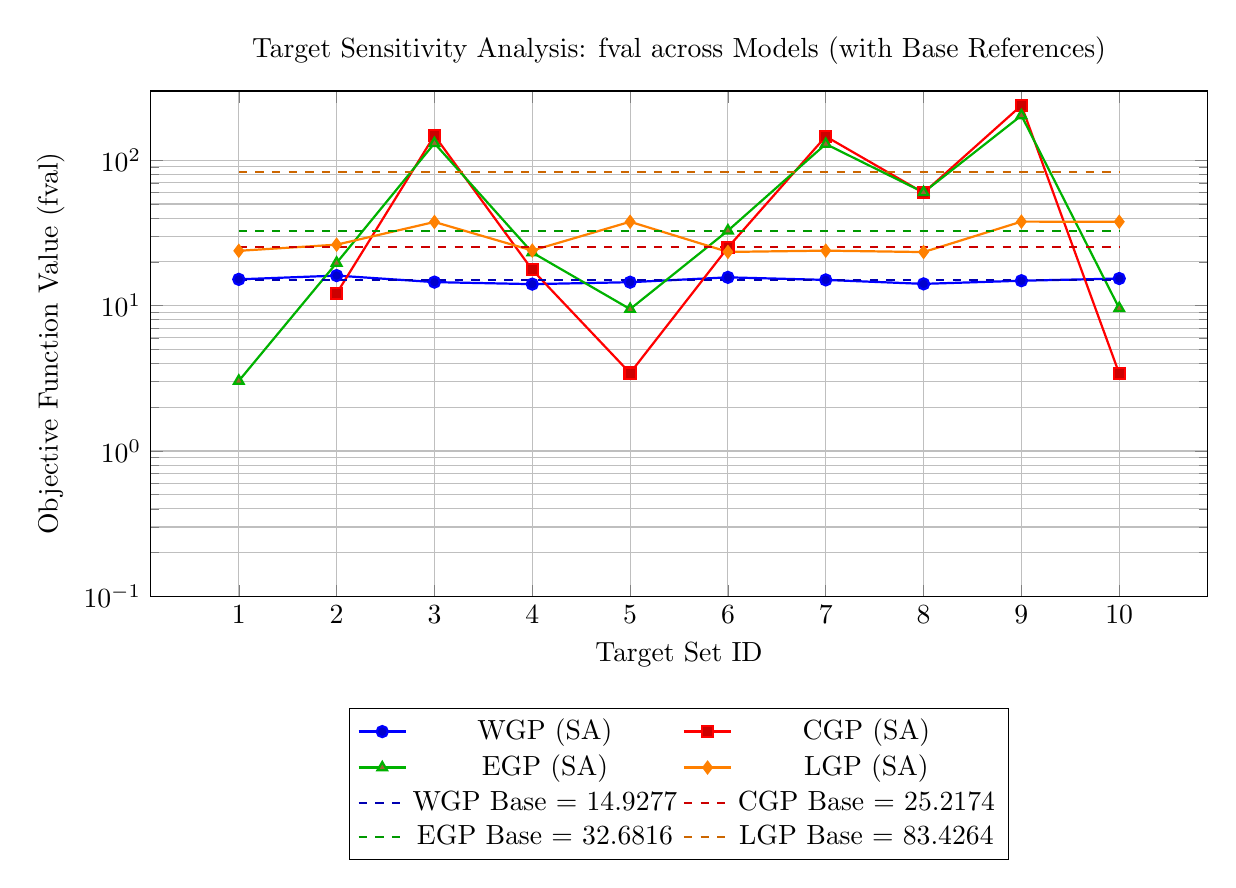
\begin{tikzpicture}
  \begin{axis}[
    title={Target Sensitivity Analysis: fval across Models (with Base References)},
    xlabel={Target Set ID},
    ylabel={Objective Function Value (fval)},
    width=15cm, height=8cm,
    xtick={1,2,...,10},
    ymin=0.1, ymax=300,
    ymode=log, log basis y=10,
    legend style={at={(0.5,-0.22)},anchor=north,legend columns=2},
    grid=both,
  ]

  % --- WGP SA ---
  \addplot+[mark=*,blue,thick] coordinates {
    (1,15.1687) (2,16.0963) (3,14.5178) (4,14.0624) (5,14.4975)
    (6,15.6563) (7,15.033) (8,14.1186) (9,14.8396) (10,15.3641)
  };
  \addlegendentry{WGP (SA)}

  % --- CGP SA ---
  \addplot+[mark=square*,red,thick] coordinates {
    (1,0) (2,12.1215) (3,148.0771) (4,17.6305) (5,3.4348)
    (6,25.1214) (7,145.9941) (8,59.7109) (9,238.5017) (10,3.404)
  };
  \addlegendentry{CGP (SA)}

  % --- EGP SA ---
  \addplot+[mark=triangle*,green!70!black,thick] coordinates {
    (1,3.0337) (2,19.6847) (3,130.949) (4,23.1993) (5,9.4657)
    (6,32.8122) (7,129.3857) (8,60.1762) (9,203.3531) (10,9.5897)
  };
  \addlegendentry{EGP (SA)}

  % --- LGP SA ---
  \addplot+[mark=diamond*,orange,thick] coordinates {
    (1,23.8339) (2,26.2725) (3,37.6495) (4,23.9389) (5,37.7732)
    (6,23.4183) (7,23.9012) (8,23.3668) (9,37.8524) (10,37.7892)
  };
  \addlegendentry{LGP (SA)}

  % --- Base reference lines (horizontal) ---
  % WGP base = 14.9277
  \addplot[blue!70!black, dashed, thick] coordinates {(1,14.9277) (10,14.9277)};
  \addlegendentry{WGP Base = 14.9277}

  % CGP base = 25.2174
  \addplot[red!80!black, dashed, thick] coordinates {(1,25.2174) (10,25.2174)};
  \addlegendentry{CGP Base = 25.2174}

  % EGP base = 32.6816
  \addplot[green!60!black, dashed, thick] coordinates {(1,32.6816) (10,32.6816)};
  \addlegendentry{EGP Base = 32.6816}

  % LGP base = 83.4264
  \addplot[orange!80!black, dashed, thick] coordinates {(1,83.4264) (10,83.4264)};
  \addlegendentry{LGP Base = 83.4264}

  \end{axis}
\end{tikzpicture} 
\caption{Target Sensitivity Analysis: \textit{fval} across target sets for WGP, CGP, EGP, and LGP with dashed lines showing Base model objective values. Logarithmic scale improves joint visibility across models.}
\label{fig:target_sa_linechart_with_base}
\end{figure}
        
\begin{figure}[htbp]
\centering
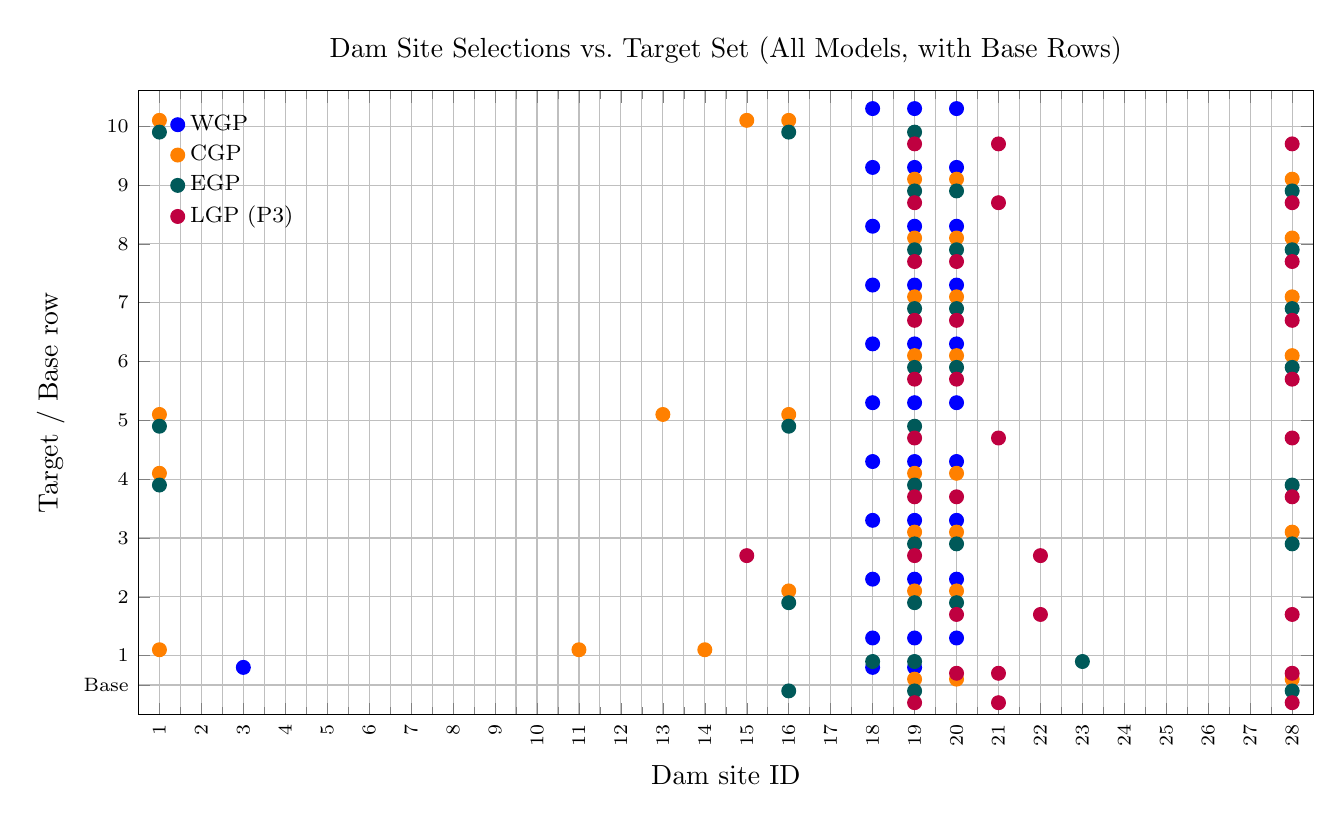
\begin{tikzpicture}
  \begin{axis}[
    title={Dam Site Selections vs.\ Target Set (All Models, with Base Rows)},
    xlabel={Dam site ID},
    ylabel={Target / Base row},
    xmin=0.5, xmax=28.5,
    ymin=0.0, ymax=10.6,
    xtick={1,2,...,28},
    ytick={0.5,1,2,3,4,5,6,7,8,9,10},
    yticklabels={Base,1,2,3,4,5,6,7,8,9,10},
    x tick label style={font=\scriptsize, rotate=90, anchor=east},
    y tick label style={font=\scriptsize},
    width=16.5cm, height=9.5cm,
    grid=both, minor tick num=1,
    legend style={at={(0.02,0.98)}, anchor=north west, draw=none, fill=none, font=\footnotesize},
    legend cell align=left
  ]

  

  % ---- Model row offsets (constant across all targets) ----
  % Base anchor row at y=0.5
  % WGP: +0.30 ; CGP: +0.10 ; EGP: -0.10 ; LGP: -0.30
  % For target set t, rows are: t+0.30 (WGP), t+0.10 (CGP), t-0.10 (EGP), t-0.30 (LGP)

  % ===================== WGP =====================
  \addplot+[only marks, mark=*, mark options={fill=blue, draw=blue}, mark size=2.5pt]
    coordinates
    % --- Base (WGP base selected: 18,19,3) at y=0.5+0.30=0.80
    {(3,0.80) (18,0.80) (19,0.80)
    % --- Target sets (always 18,19,20)
     (18,1.30) (19,1.30) (20,1.30)
     (18,2.30) (19,2.30) (20,2.30)
     (18,3.30) (19,3.30) (20,3.30)
     (18,4.30) (19,4.30) (20,4.30)
     (18,5.30) (19,5.30) (20,5.30)
     (18,6.30) (19,6.30) (20,6.30)
     (18,7.30) (19,7.30) (20,7.30)
     (18,8.30) (19,8.30) (20,8.30)
     (18,9.30) (19,9.30) (20,9.30)
     (18,10.30) (19,10.30) (20,10.30)};
  \addlegendentry{WGP}

  % ===================== CGP =====================
  \addplot+[only marks, mark=*, mark options={fill=orange, draw=orange}, mark size=2.5pt]
    coordinates
    % --- Base (CGP base: 19,20,28) at y=0.5+0.10=0.60
    {(19,0.60) (20,0.60) (28,0.60)
    % --- Target set 1: 1,11,14
     (1,1.10) (11,1.10) (14,1.10)
    % --- 2: 16,19,20
     (16,2.10) (19,2.10) (20,2.10)
    % --- 3: 19,20,28
     (19,3.10) (20,3.10) (28,3.10)
    % --- 4: 1,19,20
     (1,4.10) (19,4.10) (20,4.10)
    % --- 5: 1,13,16
     (1,5.10) (13,5.10) (16,5.10)
    % --- 6: 19,20,28
     (19,6.10) (20,6.10) (28,6.10)
    % --- 7: 19,20,28
     (19,7.10) (20,7.10) (28,7.10)
    % --- 8: 19,20,28
     (19,8.10) (20,8.10) (28,8.10)
    % --- 9: 19,20,28
     (19,9.10) (20,9.10) (28,9.10)
    % --- 10: 1,15,16
     (1,10.10) (15,10.10) (16,10.10)};
  \addlegendentry{CGP}

  % ===================== EGP =====================
  \addplot+[only marks, mark=*, mark options={fill=teal!70!black, draw=teal!70!black}, mark size=2.5pt]
    coordinates
    % --- Base (EGP base: 16,19,28) at y=0.5-0.10=0.40
    {(16,0.40) (19,0.40) (28,0.40)
    % --- 1: 18,19,23
     (18,0.90) (19,0.90) (23,0.90)
    % --- 2: 16,19,20
     (16,1.90) (19,1.90) (20,1.90)
    % --- 3: 19,20,28
     (19,2.90) (20,2.90) (28,2.90)
    % --- 4: 1,19,28
     (1,3.90) (19,3.90) (28,3.90)
    % --- 5: 1,16,19
     (1,4.90) (16,4.90) (19,4.90)
    % --- 6: 19,20,28
     (19,5.90) (20,5.90) (28,5.90)
    % --- 7: 19,20,28
     (19,6.90) (20,6.90) (28,6.90)
    % --- 8: 19,20,28
     (19,7.90) (20,7.90) (28,7.90)
    % --- 9: 19,20,28
     (19,8.90) (20,8.90) (28,8.90)
    % --- 10: 1,16,19
     (1,9.90) (16,9.90) (19,9.90)};
  \addlegendentry{EGP}

  % ===================== LGP (Priority 3) =====================
  \addplot+[only marks, mark=*, mark options={fill=purple, draw=purple}, mark size=2.5pt]
    coordinates
    % --- Base (LGP base P3: 19,21,28) at y=0.5-0.30=0.20
    {(19,0.20) (21,0.20) (28,0.20)
    % --- 1: 20,21,28
     (20,0.70) (21,0.70) (28,0.70)
    % --- 2: 20,22,28
     (20,1.70) (22,1.70) (28,1.70)
    % --- 3: 15,19,22
     (15,2.70) (19,2.70) (22,2.70)
    % --- 4: 19,20,28
     (19,3.70) (20,3.70) (28,3.70)
    % --- 5: 19,21,28
     (19,4.70) (21,4.70) (28,4.70)
    % --- 6: 19,20,28
     (19,5.70) (20,5.70) (28,5.70)
    % --- 7: 19,20,28
     (19,6.70) (20,6.70) (28,6.70)
    % --- 8: 19,20,28
     (19,7.70) (20,7.70) (28,7.70)
    % --- 9: 19,21,28
     (19,8.70) (21,8.70) (28,8.70)
    % --- 10: 19,21,28
     (19,9.70) (21,9.70) (28,9.70)};
  \addlegendentry{LGP (P3)}

  % --- A small guide on offsets (optional)
  \node[anchor=west, font=\scriptsize, align=left] at (axis cs:28.6,10.4)
    {Offsets per target row: \\
     WGP: +0.30,\ CGP: +0.10,\\
     EGP: $-0.10$,\ LGP: $-0.30$.\\
     Base row anchored at 0.5.};
  \end{axis}
\end{tikzpicture}
\caption{Selected dam sites by model and target set (circles; slight vertical offsets prevent overlap). Base models included on the “Base” row.}
\label{fig:dam_selection_targets_all_models}
\end{figure}







\begin{table}[htbp]
\centering
\caption{Descriptive statistics of $fval$ across Target Sensitivity Analysis (per model).}
\label{tab:target_sa_stats}
\begin{tabular}{lcccc}
\toprule
Model & Min & Max & Mean & Std Dev \\
\midrule
WGP & 14.06 & 16.10 & 14.93 & 0.63 \\
CGP & 0.00 & 238.50 & 65.20 & 87.44 \\
EGP & 3.03 & 203.35 & 61.46 & 71.29 \\
LGP (P3) & 23.37 & 37.85 & 29.22 & 6.21 \\
\bottomrule
\end{tabular}
\end{table}


\begin{figure}[htbp]
\centering
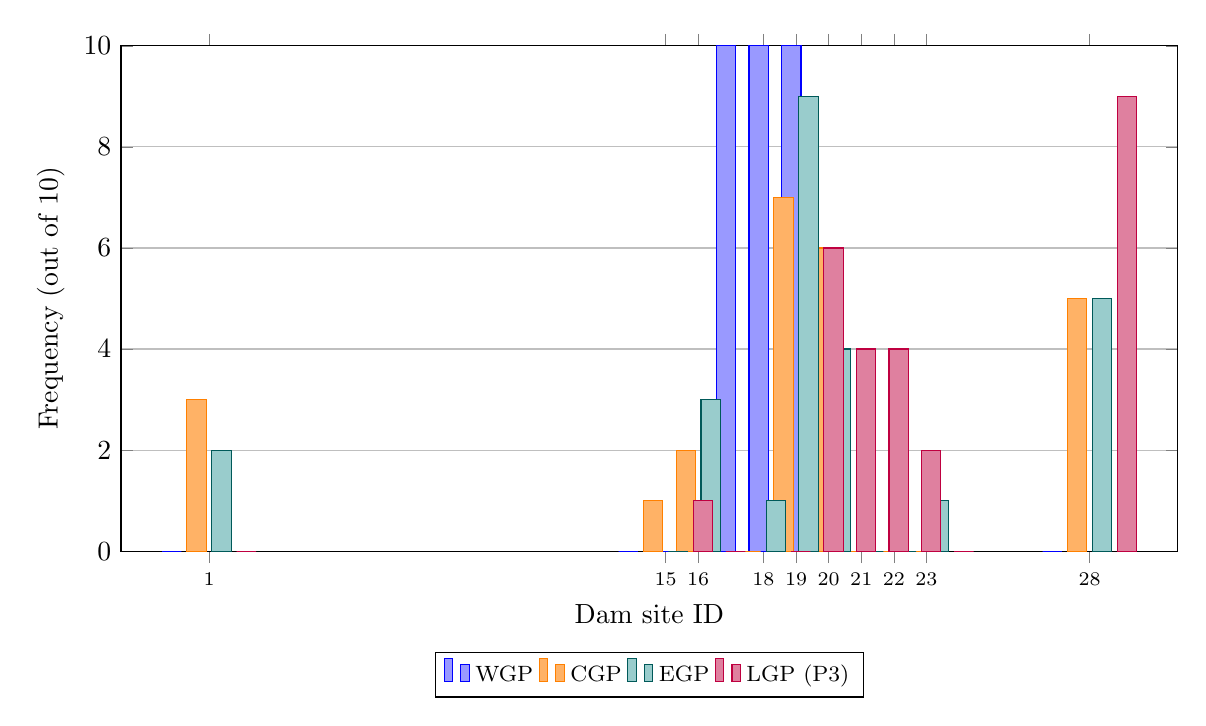
\begin{tikzpicture}
\begin{axis}[
  ybar,
  bar width=7pt,
  width=15cm, height=8cm,
  ylabel={Frequency (out of 10)},
  xlabel={Dam site ID},
  ymin=0, ymax=10,
  xtick=data,
  xticklabel style={font=\scriptsize},
  enlarge x limits=0.1,
  legend style={at={(0.5,-0.2)}, anchor=north, legend columns=4, font=\footnotesize},
  ymajorgrids,
]

% WGP
\addplot+[blue, fill=blue!40] coordinates {
  (1,0) (15,0) (16,0) (18,10) (19,10) (20,10) (21,0) (22,0) (23,0) (28,0)
};

% CGP
\addplot+[orange, fill=orange!60] coordinates {
  (1,3) (15,1) (16,2) (18,0) (19,7) (20,6) (21,0) (22,0) (23,0) (28,5)
};

% EGP
\addplot+[teal!70!black, fill=teal!40] coordinates {
  (1,2) (15,0) (16,3) (18,1) (19,9) (20,4) (21,0) (22,0) (23,1) (28,5)
};

% LGP
\addplot+[purple, fill=purple!50] coordinates {
  (1,0) (15,1) (16,0) (18,0) (19,6) (20,4) (21,4) (22,2) (23,0) (28,9)
};

\legend{WGP, CGP, EGP, LGP (P3)}

\end{axis}
\end{tikzpicture}
\caption{Selection frequency of dam sites across Target Sensitivity Analysis (only sites selected at least once).}
\label{fig:target_sa_barplot_filtered}
\end{figure}







